\chapter{Regularization}

Deep Neural Networks tend to represent very complex functions which leads to overfitting the training data (variance in the estimator). Therefore, most regularization strategies are based on regularizing estimators which trades bias for a reduced variance. Additionally, regularization will also reduce the capacity of the model. The learning bias will favour simpler hypothesis.

\section{Parameter Norm Penalties}

We can perform regularization by adding a parameter norm penalty $\Omega(w)$ that limits the capacity of the model to the cost function J.

$$ J(w, X, y) + \alpha \Omega (w) $$

Where $\alpha$ is a hyper-parameter that weights the relative contribution of the norm penalty term, $\Omega$ relative to the standard cost function J. A larger $\alpha$ then will result in more regularization.

\begin{figure}[h]
    \centering
    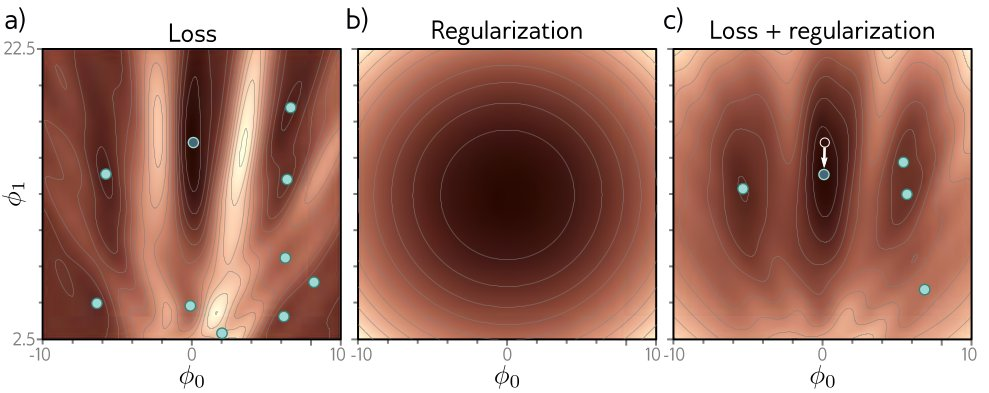
\includegraphics[width=12cm]{Images/parameter-norm.jpg}
    \label{fig:parameter-norm}
\end{figure}

\subsection{L2 Parameter Regularization}

The L2 parameter norm penalty, also known as weight decay drives the weights closer to the origin by adding a regularization term to the cost function.

$$ \Omega(w) = \frac{1}{2} || w ||_{2}^{2} $$

\noindent If we remember, Maximum Likelihood Estimator was an special case of Maximum a Posteriori Estimation when we had a uniform prior. By adding a regularization parameter to the cost function we are changing the prior distribution to a Gaussian prior centered on 0 where the hyperparameter $\alpha$ acts like the variance. In this way we are favouring the hypothesis inside our hypothesis space that have smaller weights.

\newpage
\noindent Performing the gradient adding to the cost function the L2 norm is known as ridge regression or Tikhonov regularization. 

$$\Tilde{J} (w, X, y) = \frac{\alpha}{2} w^T w + J(w, X, y) ~~~~~ \nabla_w \Tilde{J} (w, X, y) = \alpha w + \nabla_w J (w, X, y)$$

\noindent The addition of the weight decay term will modify the learning rule to shrink the weight vector by a constant factor on each step, just before performing the usual gradient update.

$$ w \leftarrow w - \epsilon \left( \alpha w + \nabla_w J(w, X, y) \right) ~~~~~  w \leftarrow (1 - \epsilon \alpha) w - \epsilon \nabla_w J(w, X, y) $$

\subsection{L1 Parameter Regularization}

Another option is to use L1 regularization which is defined as:

$$ \Omega (w) = ||w||_1 $$

\noindent In comparison to L2 regularization, L1 regularization results in a solution that is more sparse. Sparsity refers to the fact that some parameters have an optimal value of zero making L1 regularization fitting for use in feature selection.

\noindent The gradient now will be.

$$ \nabla_w  \Tilde{J} (w, X, y) = \alpha sign(w) + \nabla_w J (w, X, y)$$

Notice how the weights $w$ are pushed to 0 by adding $\alpha sign(w)$ to the gradient.




\begin{figure}[h]
    \centering
    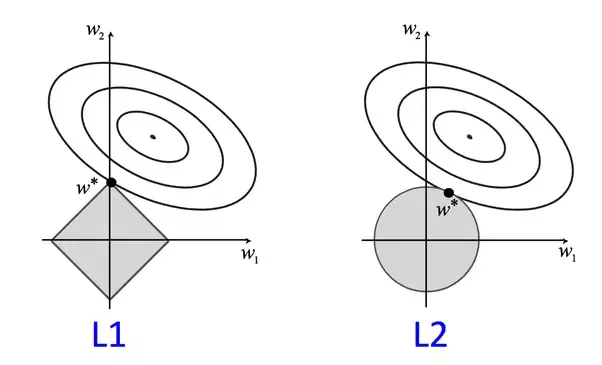
\includegraphics[width=6cm]{Plots/parameter_regularization.png}
    \caption{L1 and L2 regularization behaviour}
    \label{fig:parameter-regularization}
\end{figure}

\section{Other Regularization Techniques}

\subsection{Data Augmentation}

The best way to make a model generalize better is to train it on more data. In case we cannot gather more data, we can apply a small transformation to the training data generating fake data in the process which we will be able to add it to the training set. This technique is called data augmentation. Dataset augmentation has been particularly effective for object recognition. Creating new samples rotating, translating or scaling our images will ensure that the model is invariant to rotations, translations and scaling transformations making it to generalize better.


\subsection{Transfer Learning (Pre-training)}

Transfer learning is a regularization technique used when the training data is limited. It involves training a neural network on a related secondary task for which data are more plentiful. The network learns valuable features from this secondary task, which can later be utilized to improve performance on the original task. Basically, transfer learning can be seen as initializing most of the parameters of the final network in a sensible part of the space that is likely to produce a good solution.

\newpage

\subsection{Multi-task Learning}

Multi-task learning involves training a single neural network model using examples from multiple related tasks. The model then will have both task-specific and generic parameters. The shared layers captures common patterns and makes the model able to learn a representation that generalizes well.
Meanwhile, the task-specific layers handle task-specific details. Multi-task learning improves performance by leveraging knowledge from multiple tasks and benefiting from shared representations.

\begin{figure}[htp]
    \centering
    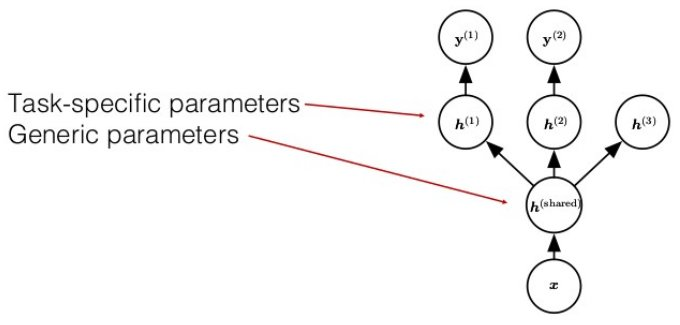
\includegraphics[width=10cm]{Images/multi-task_learning.jpg}
    \caption{Multi Task Learning}
    \label{fig:muti-task_learning}
\end{figure}

\subsection{Self-Supervised Learning}

When data from other tasks is not available, self-supervised learning can be used to create large amounts of “free” labeled data and use it for transfer learning. There are two types of self-supervised learning: Generative and Constrastive.

\begin{itemize}
    \item Generative Self-supervised Learning: Part of each data sample is masked and the secondary task is predicting missing parts in masked data.
    \item Constrastive Self-supervised learning: Two versions of each unlabeled example are presented, where one has been distorted in some way. The system is then trained to predict which is the original.
\end{itemize}

\noindent These techniques help the network learn representations that can be transferred to the primary task, enhancing performance without task-specific labeled data.

\begin{figure}[h]
    \centering
    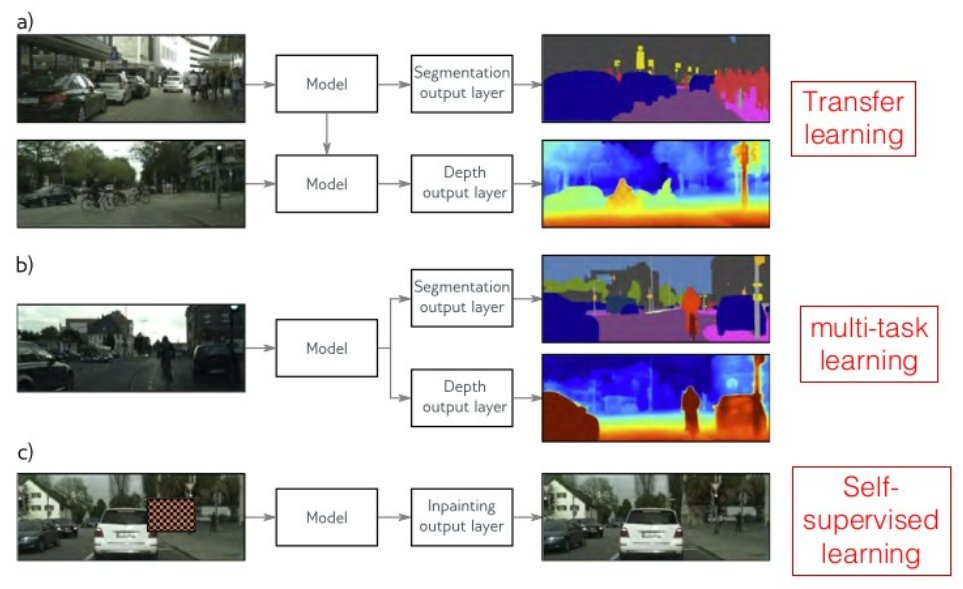
\includegraphics[width=13cm]{Images/self-supervised_learning.jpg}
    \caption{Self-Supervised Learning}
    \label{fig:self-supervised}
\end{figure}

\subsection{Early Stopping}

When training large models these ones may overfit as the number of epochs go by. We often observe that training error decreases steadily over time, but the validation set error begins to rise again.

\begin{figure}[htp]
    \centering
    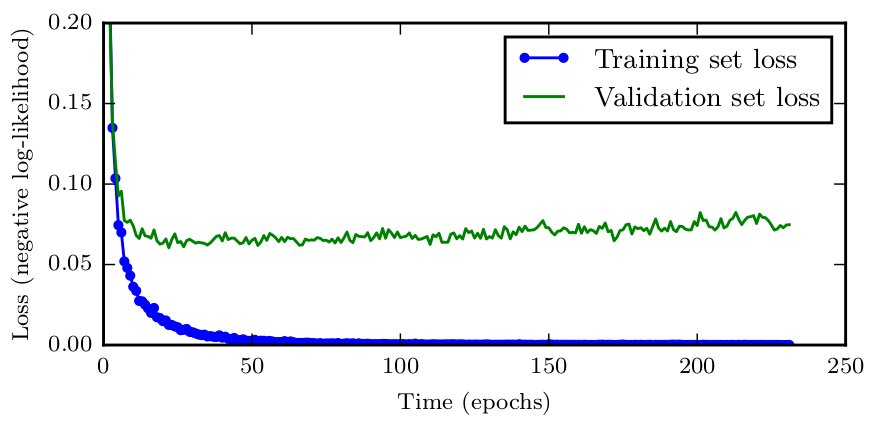
\includegraphics[width=7.5cm]{Plots/early-stopping.jpg}
    \caption{Early Stopping}
    \label{fig:early-stopping}
\end{figure}

\noindent What we can do is to stop the training algorithm once we see no improvement for N epochs. This technique is called early stopping. We will therefore regularize the model as it limits the parameter space to a neighborhood of the initial parameter values.

\subsection{Bagging and Boosting}

Bagging is a technique for reducing generalization error by combining several models. The idea is to train several different models separately with different subsets of the data through sampling with replacement, then have all of the models vote on the output for the test examples. On the other hand, boosting works in the opposite direction. Instead of reducing variance, boosting builds an ensemble with higher capacity. In boosting, each model is trained iteratively, with subsequent models focusing on the examples that were previously misclassified by earlier models. By giving more weight to difficult examples, boosting aims to improve the overall performance of the ensemble. Examples: AdaBoost and XGBoost. Training different models and using ensembles, such as bagging and boosting, improve performance by reducing errors and increasing model diversity.


\begin{figure}[h]
    \centering
    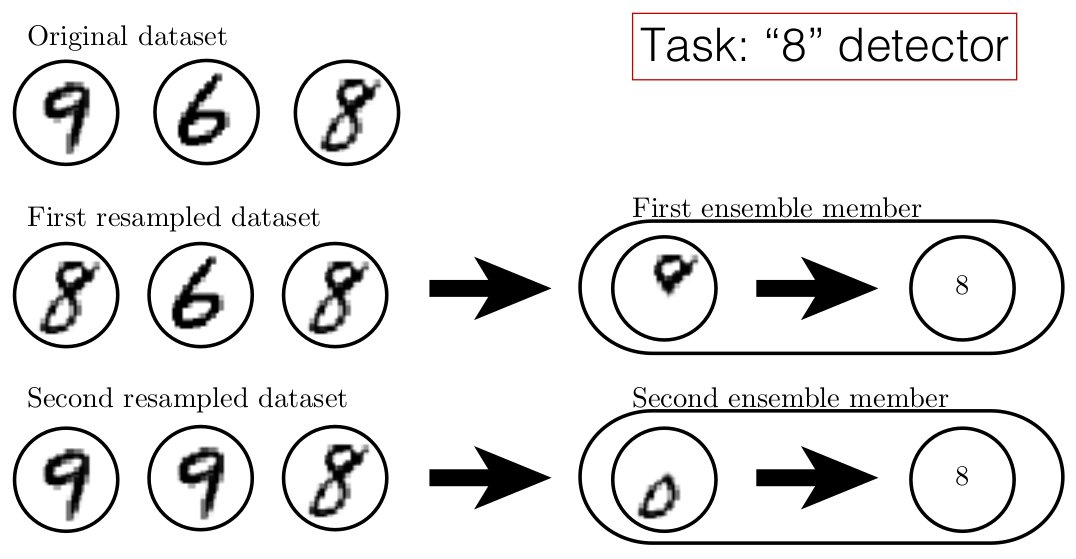
\includegraphics[width=10cm]{Images/bagging.jpg}
    \caption{Caption}
    \label{fig:bagging}
\end{figure}

\newpage
\subsection{Dropout}

Dropout is an efficient regularization technique used in Neural Networks that involves randomly removing units from the network during training using binary masks which silences some neurons. This creates an ensemble of sub-networks. Therefore, dropout can be seen as a way to perform an ensemble method on a Deep Neural Network. Each sub-network inherits a different subset of parameters from the parent network. This process approximates the idea of training multiple independent models in bagging. Basically, we reduce the generalization error by combining several models. The idea is to train several different models separately, then have all of the models vote (or take the mean of them) on the output for the test examples. This process helps in reducing overfitting and introducing regularization to the network.

\begin{figure}[h]
    \centering
    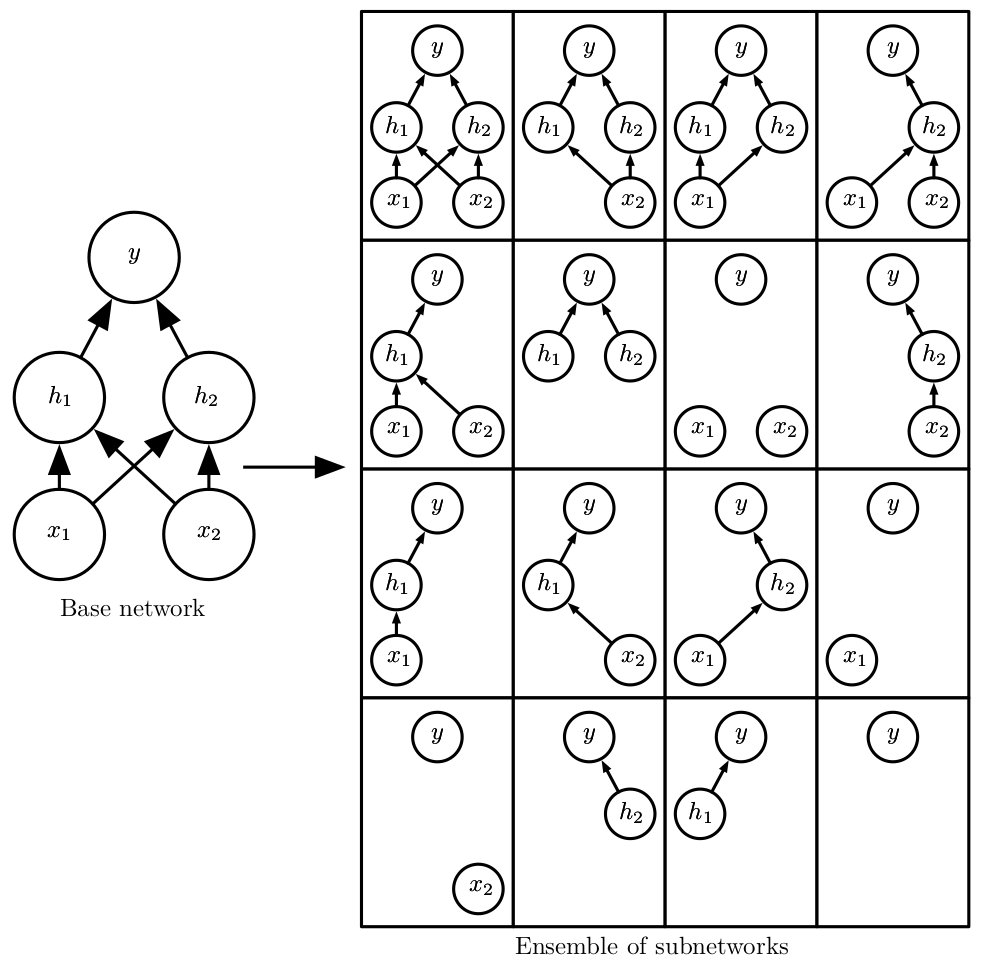
\includegraphics[width=10cm]{Images/dropout.jpg}
    \caption{Dropout ensemble of networks}
    \label{fig:dropout}
\end{figure}

\noindent Dropout then is able to reduce overfitting by considering simpler models of our DNN but constructing many of them so the errors of one model will not be repeated by the others. This is a strategy to reduce the variance of the NN trading it with bias.

\noindent During evaluation, dropout is not applied. Instead, the full network is used for predictions. However,
the weights of the neurons are scaled down by the dropout probability to account for the fact that,
on average, fewer neurons were active during training. This scaling ensures that the expected output
of the neurons remains the same, maintaining consistency between training and evaluation.

\newpage
\subsection{Adversial Training}

Adversarial training introduces adversarial samples that are intentionally crafted input data slightly perturbed to mislead the model’s prediction. These are samples constructed by using an optimization procedure to search for an input $x'$ near a data point $x$ such that the model output is very different at $x'$.

\begin{figure}[h]
    \centering
    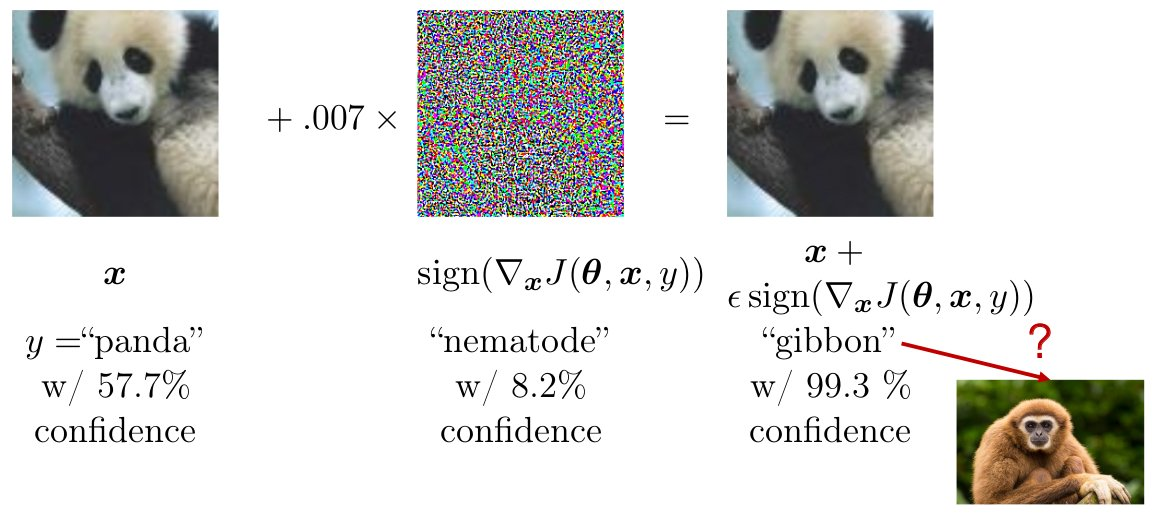
\includegraphics[width=12cm]{Images/adversarial-training.jpg}
    \caption{Caption}
    \label{fig:enter-label}
\end{figure}

\noindent The addition of adversarial examples introduces a form of regularization by effectively expanding the training distribution to include adversarial instances. This helps prevent overfitting in the training set and encourages the model to learn more robust and generalizable features.


